% ============================================================================
% Barycentre de deux points ponderes : G = bar{(A;2),(B;3)}
% Extrait de la fiche : Barycentres et lignes de niveau (classe de 1ere D)
% Necessite \usepackage{tikz} et \usetikzlibrary{calc} (charges par le fichier principal)
% ============================================================================
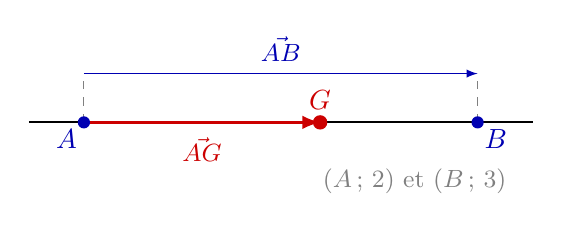
\begin{tikzpicture}[scale=1.0,>=latex]
  \coordinate (A) at (0,0); \coordinate (B) at (5,0); \coordinate (G) at (3,0);
  \draw[thick] (-0.7,0) -- (5.7,0);
  \draw[->,thin,blue!70!black] (0,0.62) -- (5,0.62) node[midway,above=1pt,font=\small] {$\vec{AB}$};
  \draw[gray,dashed] (0,0) -- (0,0.62); \draw[gray,dashed] (5,0) -- (5,0.62);
  \draw[->,very thick,red!80!black] (A) -- (G);
  \node[red!80!black,font=\small,fill=white,inner sep=1pt] at (1.5,-0.35) {$\vec{AG}$};
  \fill[blue!70!black] (A) circle (2.2pt) node[below left=-1pt] {$A$};
  \fill[blue!70!black] (B) circle (2.2pt) node[below right=-1pt] {$B$};
  \fill[red!80!black] (G) circle (2.6pt) node[above=1pt] {$G$};
  \node[font=\small,gray] at (4.2,-0.75) {$(A\,;\,2)$ et $(B\,;\,3)$};
\end{tikzpicture}
